
%----------------------------------------------------------------------------------------
%	PACKAGES AND OTHER DOCUMENT CONFIGURATIONS
%----------------------------------------------------------------------------------------

\documentclass[11pt]{article} % Default font size is 12pt, it can be changed here

\usepackage{geometry} % Required to change the page size to A4
\geometry{a4paper, margin=2cm} % Set the page size to be A4 as opposed to the default US Letter

\usepackage{graphicx} % Required for including pictures

\usepackage{float} % Allows putting an [H] in \begin{figure} to specify the exact location of the figure

\usepackage{cite}

\begin{document}
	
	\title{Reading Project: Industrial Mathematics }
	\author{Margaret Duff }
	\date{Today}
	\maketitle
	
	\begin{abstract}
		Industrial Maths is.......
	\end{abstract}
	\tableofcontents 
	
	\section{Introduction}
	
	\section{Review of the International State of Industrial and Applied Mathematics, Mechanisms, Philosophy and Effectiveness}
	
	This report will mainly be  focused on the UK but we will look elsewhere in the world for examples and comparisons. 
	\subsection{Definitions} 
	
	Defining the language and descriptors of  Industrial Maths is not a simple task indeed many writers choose a range of definitions. 
	
	Even defining what it means to do Mathematical Research is fraught with complications. One can't just count all those employed by universities and higher education institutes as there are a large number of very talented mathematicians working elsewhere. 	Deloitte in their report 'Measuring the Economic Benefits of Mathematical Science Research in the UK' \cite{deloitteuk} count 'Mathematical Science Occupations' as those 'which either entail mathematical science research, or used mathematical science research-derived tools and techniques' a broad definition which includes individuals which need no understanding of the underlying tools or techniques an includes all hospital and healthcare managers, social science researchers and public service administrative professionals. All very valuable jobs but not ones that I would put in the category of 'Mathematical Science Occupations. 
	In a similar report Doloitte produced on the Dutch economy \ref{deloittedutch} they narrow this definition slightly by considering ' only people in jobs requiring a higher education' to be included.  A better but still quite broad definition.
	One might suggest those people who currently use or research 'modern' mathematical science research tools, to avoid including all those people that use an excel spreadsheet to add up large numbers. But then the definition of modern is fraught, MORE HERE
	For the purpose of this report, I  will consider Mathematics to be that which is of interest to academic mathematicians. Mathematics focuses on the underlying structure and pattern, looks for generalisations and derives exact or approximate solutions backed up by logical proof. The important clarification is that the application of well known techniques does not count. 
	
	
 Defining Industry is perhaps simpler as I define it be any non-mathematical institution including: governments, businesses, manufacturers, other academic departments, hospitals, schools, charities etc. 


		For industrial mathematics, we could perhaps use words such as: 'applicable', 'interdisciplinary, 'applied', 'knowledge transfer' or 'mathematics communication'. The Bond Report \cite{Bond} describes '\textit{Impactful Mathematics} as any mathematical method that has practical application and generates societal and/or economic value'. 
		
		For this report I will use the definition John Stockie describes in his essay 'Mathematics for Industry A personal Perspective' \cite{Stockie2015} that Industrial Mathematics includes: 
		
	\begin{itemize}
	\item mathematics that is done by non-academic mathematicians who work as employee of a company
	\item mathematics that is done by academic mathematicians within research institutions for a company, or in collaboration with a company
	\item mathematics that is inspired by industry and arise from an industrial setting. 
	\end{itemize}
	
	
	John Stockie essay \cite{Stockie2015}.
	\subsection{Significance}
	Deloitte Report
	
	Dutch Deloitte Report 
	\subsection{Mechanisms}
	European Study Groups in Industry 
	
	Some study group reports 
	
	Innovate UK /Knowledge Transfer Network 
	
	Smith institute
	
	Canadian examples - CQAM, Fields 
	\subsection{Successes}
	BOND Review 
	
	Women in industrial maths?? 
	\subsection{Challenges} 
	BOND Review
	
	\subsubsection{Identifying Suitable Problems and Creating links} 
	Especially SMEs 
	\subsubsection{Building working relationships}
	A long process!!!!
	Intellectual Property issues 
	\subsubsection{Funding} 
	Talk about Bond Review and about 100 phd student places etc., boosting of EPSRC funding etc. 
	\subsubsection{Academic Career Paths} 
	Needs to be seen as a viable career option 
	How to prevent people being snaffled to industry 
	\subsubsection{Brexit}
	I am reluctant to mention the 'B' word but i think no report that looks at the future of Mathematical Research, Industry or Mathematics in Industry can avoid the topic. The whole scientific community is concerned over the future of funding and ability to collaborate (BREXIT LETTER NOBEL LAUREATES) and industry in the UK is facing an uncertain future (REFERENCE OR MORE HERE).
	
	I don't want to spend much time on this, but I would like to say that whatever happens, examples of success stories in industrial mathematics have demonstrated the need for collaboration: with industry, with other fields, with other departments and it will be vital for the continuing success of Industrial Mathematics that the spirit of collaboration is maintained. 
	
	\subsection{Case Study 1: Trip Wire Detection for Land Mines}
	
	The first case study that really stood out to me, was one brought to the second Industrial Problem-Solving Workshop (a Canadian version of the ESGI) held in Calgary in 1998. I follow an account of the project by one of the attendees, John Stockie \cite{Stockie2015} and the Study Group report \cite{Jessop}.
	
The industrial partner was ITRES Research LTD and they were experimenting mounting a detection camera on a boom ahead of a slowly moving truck which would look vertically downwards. It was hoped that an automatic algorithm would be used to find trip wires appearing in the image. 
	
	A report, the Landmine Monitor, produced in 1999 \cite{landmine} suggests that at the time the of the Study Group there were more than 250million Anti-personnel Mines in Stockpiles of which they were particularly concerned about remotely-delivered, surface laid anti vehicle mines that utilize trip wires which could explode from innocent acts by individuals. 
	
	A clearly defined  problem, that could have huge benefits worldwide so why was this a study group problem? Why hadn't a solution been implemented already? There were some inherent difficulties in detecting a tripwire including:
	\begin{itemize}
	\item wires are often partially covered by foliage
	\item wires are not uniform in illumination 
	\item wires are often purposefully camouflaged and come in a variety of colours and transparencies
	\item other image features may mimic lines such as vegetation 
	\item images are often noisy or blurry as trucks and cameras move or the camera fails to focus. Natural elements also cause additional artefacts in the field of view
	\end{itemize}
	The goal of the week long study group was to have a first attempt at developing an algorithm that was \textsl{robust} enough to cope with the problems above; \textit{reliable }enough to detect trip wires in with near perfect sensitivity and a high specificity and to be \textit{fast} enough to run before the truck detonates a landmine. 
	
	We will look at 3 elements of their work: pre-processing, line detection and improving speed:
	\paragraph{Pre-processing}
\begin{itemize}
	\item \textbf{Laplacian Filter}: Mathematicians love definitions and in this case careful consideration of the definition of a wire in an image indicates a possible direction of work. Defining image intensity to be a function $u(x,y)$ of position $(x,y)$ and thus a line, a sharp edge, is one in which the function $u(x,y) $ has a high curvature.
	To enhance this feature the convolution of the image with a Laplacian filter is taken. This has a similar effect to taking the second derivative and accentuates regions of high curvature.	
	\item \textbf{Edge detection }: Edges are then found in the filtered image using either the Sobel edge detector or the log method. The result is a binary image with found edges indicated. 
	\end{itemize}
	
	\paragraph{Line Detection}
	Continuing the theme of precise definitions: the differentiating factor between any old line and a potential trip wire is that a wire is locally straight and although could be partially hidden consists of a sequence of co-linear line segments. In order to detect such lines they use: 
		\begin{itemize}
		\item \textbf{Radon Transform}: The Radon transform of a 2D image given by:
		
		\begin{equation}
			R(\rho, \theta)=\int_{R^2} u(x,y)\delta(x\cos(\theta)+y\sin(\theta)-\rho) dx dy 					
		\end{equation}
		transforming the image from an $(x,y) $ domain to a $ (\rho, \theta)$ domain. Peaks in the $ (\rho, \theta)$ domain correspond to lines of the form $ x\cos(\theta)+y\sin(\theta)=\rho$ in the $(x,y) $ domain. 
		\item \textbf{Threshold transformed images }: Finding the peaks in the $ (\rho, \theta)$ domain requires some sort of threshold. If the threshold is too high then no wires are found, too low and there are too many false positives. What is defined as a wire is independent of individual images but variations in images can cause additional noise inflating all the values in the $ (\rho, \theta)$ domain causing issues. This is not a simple issue. 
	\end{itemize}
	\paragraph{Algorithm Speed}
		\begin{itemize}
		\item \textbf{Using the FFT}: A the time of the Study Group Matlab's inbuilt Radon transform did not take advantage of the fast Fourier transform to speed up implementation. Such a possibility was discussed. 
		\item \textbf{Exploiting the method of image acquisition}: Images are received from the camera as a sequence of lines that are constantly updated. Discussion was had as to how the intensities in the $ (\rho, \theta)$ domain can be continuously updated as each new line is attained, reducing the number of computations compared to repeatedly taking the radon transform of the whole image. 
	\end{itemize}
	
	The algorithm produced during the week was in no way perfect, struggling with some of the more 'difficult' images and ones where the wires were oblique. Results were presented to the industry partner but future collaboration was not forthcoming, a shame but potentially due to the military applications of such work. There is evidence that ITRES continued working on this problem with conference proceedings released in 2000 \cite{Babey}. \emph{TO READ THIS PLEASE!!!!!!!!}
	

	
	
	\subsection{Case Study 2 - Shelter: Homeless Populations}
	
To READ https://www.gov.scot/binaries/content/documents/govscot/publications/research-publication/2018/06/health-homelessness-scotland/documents/00536908-pdf/00536908-pdf/govscot\%3Adocument
	
   Brought to ESGI 29, held in Oxford in March 1996 a problem from the charity Shelter to model the numbers of homeless and non-homeless people in a Borough. The model should then be able to predict changes in homeless populations as a result in changes of local policy. I follow the report produced at the end of the study group \cite{Shelter1996}
	
	The populations was split into broad classes: 
	\begin{itemize}
		\item $ T= $ N umber of households in temporary accommodation (Homeless)
		\item $  P= $ Number of households permanently resident in council housing stock
		\item $ G= $ Number of households in private sector accommodation 
	\end{itemize}
	This is then further subdivided as:
	\begin{itemize}
		\item $ P_R= $ Number of households in council stock and not  seeking transfer to other council housing stock 
		\item $ P_N= $ Number of households in council stock and seeking transfer 
		\item $ G_R= $ Number of households in private sector accommodation seeking transfer to council housing stock 
		\item $ G_N= $ Number of households in private sector accommodation and not seeking transfer
	\end{itemize}

Hence we have the following relations 
\begin{itemize}
	\item $ P=P_R+P_N $
	\item $ G=G_R+G_N $
	
\end{itemize}

Also define: 
\begin{itemize}
	\item Number of Households on the register,$  R=T+P_R+G_R $
	\item $ P_0 = $ Total availability of housing stock 
	\item $ G_0= $ Total number of households in the Borough
\end{itemize}

The flows in and out of population groups are shown in Figure \ref{fig:homelessrates}. A few assumptions about negligible flows have been assumed to simplify the problem: it is assumed that homeless families only come form the private sector and also that flows from $ G_R $ to $ G_N $ and $ T $ back to $ G $ are negligible. 

This gives a system of differential equations
\begin{eqnarray}
\frac{dG_N}{dt}=-k_5 G_N-k_3 G_n +k_6 P\\
\frac{dG_R}{dt}=-k_5 G_R +k_3 G_N -k_4 (P_0-P)G_R\\
\frac{dT}{dt}=k_5 G -k_1(P_0 -P)T\\
\frac{dP_N}{dt}=-k_6 P_N -k_7 P_N +(P_0-P)(k_4 G_R +k_1 T+k_8 P_R)\\
\frac{dP_R}{dt}=-k_6 P_R+k_7 P_N -k_8(P_0-P)P_R
\end{eqnarray}
	 \begin{figure}
	 	\centering
	 	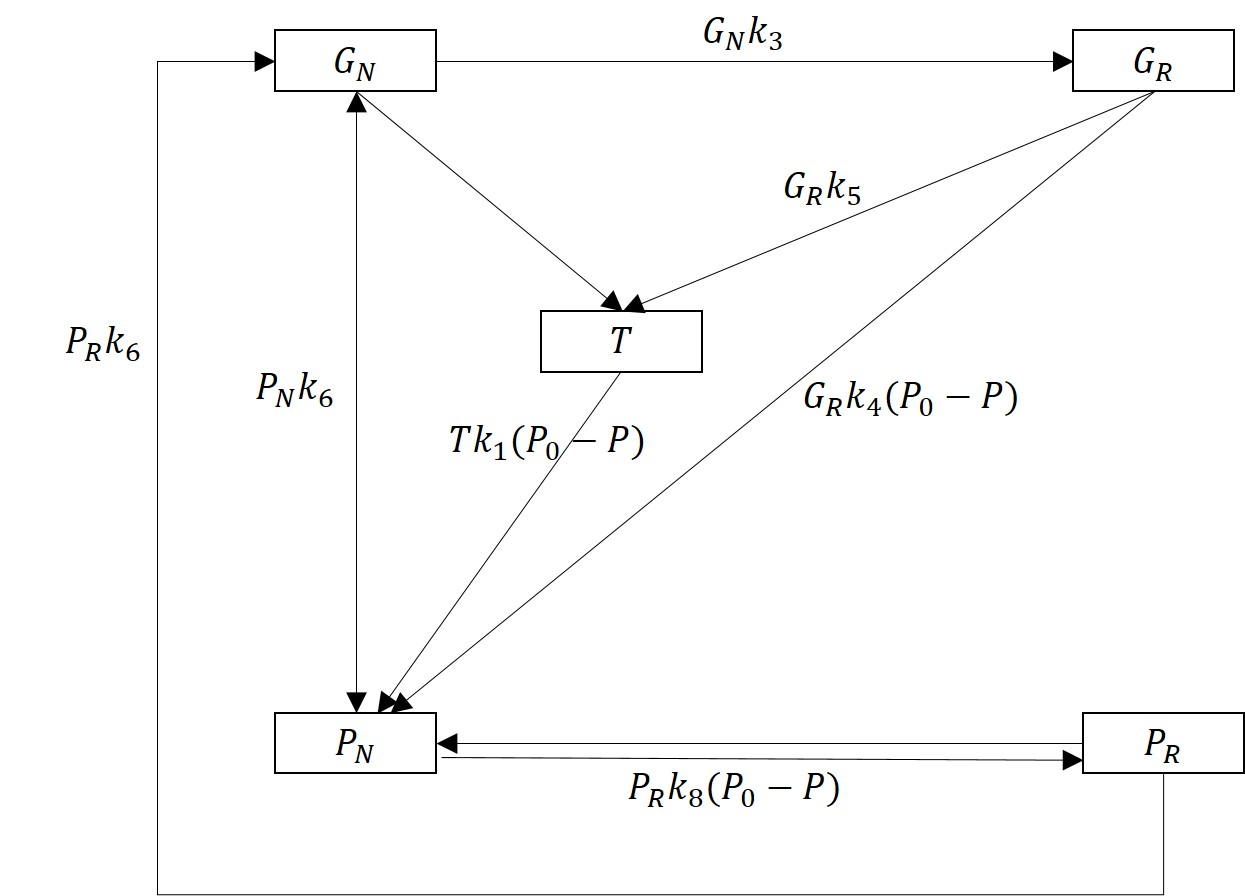
\includegraphics[width=0.7\linewidth]{Report_images/homeless_rates}
	 	
	 	\caption{A diagram to show  flows and and associated rates of households moving  between population groups}
	 	\label{fig:homelessrates}
	 \end{figure}
	 
	These equations implicitly assume that:  
	\begin{itemize}
		\item Birth and death rates can be neglected
		\item No migration in and out of the borough 
		\item Rates depend only on the present circumstances there is no delay e.g. due to administrative processes 
	\end{itemize}

These equations look intractable but substituting $ G_0=P+T+G_r+G_N $ and $ G_0=G+P+T$ reduces the system to 3 differential equations:

\begin{eqnarray}
\frac{dT}{dt}=k_5 G -k_1(P_0 -P)T\\
\frac{dG_R}{dt}=-k_5 G_R+k_3(G_0-P-T-G_R)-k_4(P_0-P)G_R\\
\frac{dP}{dt}=-k_6P+(P_0-P)(k_4G_R+k_1T)
\end{eqnarray}
	
	They looked for equilibrium solutions, so setting the left hand side of the equations to zero. They were able to see that a feasible equilibrium solution always exists, where the number of occupied council houses is positive but no greater than the number actually available. 
	
	Looking for analytic solutions of the equations in full generality was deemed unproductive for the short intensive time available in a Study group so focus was moved to looking for numerical solutions. 
	
	Initial values were chosen to represent a typical metropolitan borough. calculations were carried out with numbers of people rather than families. They found that the steady state solution was locally stable but that the values showed high sensitivity from the initial data and values. Thus generalised discussion about results for the "typical" borough or for all boroughs is not possible. They did however manage to make some useful inferences: 
	

	\begin{itemize}
		\item The populations only settle down to the steady state values over a period of about 30 years. This is a much larger time frame than changes in local and national policies and is large enough that births, deaths and migration should be taken into account. Future work should either aim to increase the complexity of the model to take this into account or should look closer at the initial dynamics and variation. 
		\item Reducing the constant $ k_1 $ by a factor of 10, signifying a change in policy so that much less priority is giving to the homeless on council waiting lists causes very little change apart from a 10-fold increase in the numbers of homeless in the borough. The amount of vacant council property increased a little but not sufficiently to cope with the increase in homeless families. The factor $ k_1 $ is important. 
	\end{itemize}
	
	FUTURE WORK??????
	
	\subsection{Case Study 3: Optimisation of the “118” Emergency Management System in Milan  }
	The book "European Success Stories in Industrial Mathematics" \ref{Lery2011} contains a wealth of great examples of effective knowledge transfer and collaboration. One particular example, "Optimisation of the "118" Emergency Management System in Milan" attracted me because of its real-world importance and clear mathematical optimisation problem but also because of a particular sentence: 
	
	\begin{quote}
		''In spite of being developed by academic personnel, the outcome of the project has been actually implemented''
	\end{quote}

	Perhaps, not a sentence I should have taken out of context, but CONTINUE HERE 
	
	

	I follow the 2013 paper by R. Arinhieri, G. Carello and D. Morale \cite{Aringhieri2016}  to describe this case study.
	
	
	\subsection{Case Study 4: Mathematical Modelling of the Dynamics of Meningococcal Meningitis in Africa  }
The book "UK Success stories in Industrial Mathematics" \cite{Aston2016} is a collection of cases studies selected from those Impact Case Studies submitted to the 2014 Research Excellence Framework. They are seen as shining examples of the mathematical sciences community engaging with problems and organisations outside of academia. 36 problems were selected out of the 250 submitted for the REF and I aimed to pick just one to write up as a case study- a challenge indeed!


The African meningitis belt spans sub Saharan Africa and see periodic fluctuations of meningococcal meningitis, cases appearing every dry season, drop off over the rainy season and a major epidemic emerges every 6-14years. Across the world, meningitis causes about 135,000 deaths annually and substantial data is available across the African meningitis belt, so mathematical modelling of epidemiology of meningococcal meningitis could lead to substantial benefits. Indeed, modelling has been attempted by a number of groups but we follow the work by K.B.Blyuss at the University of Sussex described in "UK Success stories in Industrial Mathematics." and the associated paper \cite{Irving2012}.


\paragraph{Initial Modelling and Identification of Reproduction Number  }
Looking for a simple model the team looked towards the standard SIR model. In the case of meningitis, individuals can be carriers without developing the infection and there is a high ratio of carriers to cases, thus an additional "carrier" class was a necessary addition, giving 4 classes: 
\begin{itemize}
	\item S= Susceptible
	\item C=Carriers
	\item I=Infected
	\item R=Recovered
\end{itemize}
The total population is $ N=S+C+I+R $. The question of temporary immunity was a major part of this work and they considered a variety of models where there was:
\begin{itemize}
	\item no immunity, and thus no recovered class, recovered individuals went straight  to susceptible 
	\item   immunity only if they have had developed a meningitis infection, if individuals had only been a carrier then they got new immunity
	\item immunity if they had been a carrier, developed the infection or both
\end{itemize}

\begin{figure}
	\centering
	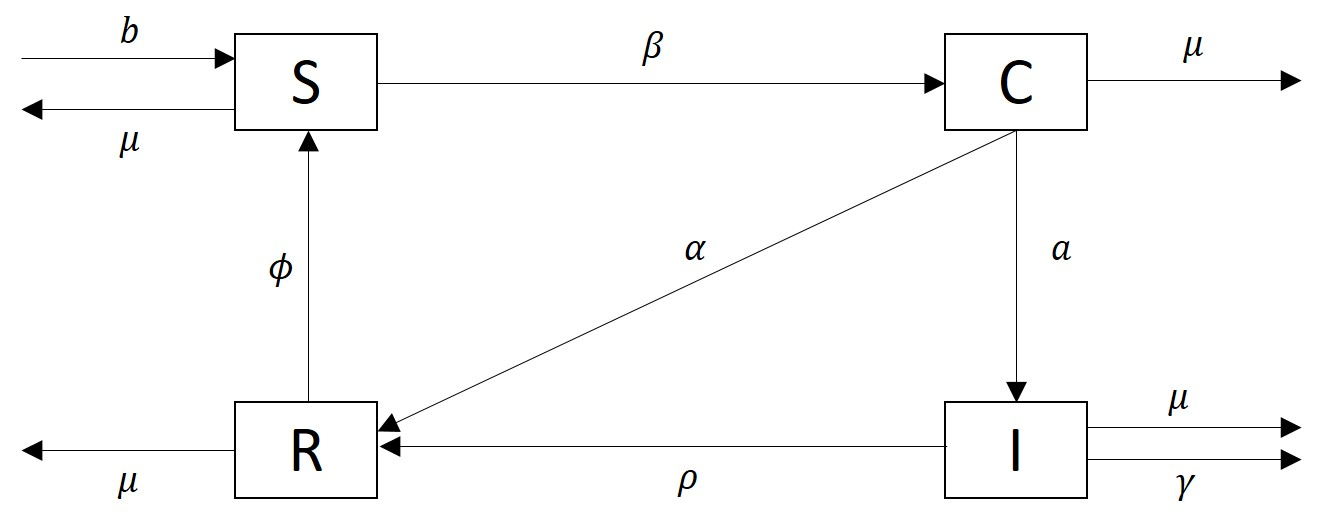
\includegraphics[width=0.7\linewidth]{Report_images/meningitis_model}
	\caption{A diagram to show the flows between population groups in the chosen meningitus model, taken from Fig 2 in paper  \cite{Irving2012}}
	\label{fig:meningitismodel}
\end{figure}



 Modelling all 3 cases they found the best fit to the observed data was the last case and the model shown in Figure \ref{fig:meningitismodel}, with rates defined as followed:
\begin{itemize}
	\item $ \beta =$ the transmission rate
	\item $ a= $ the rate at which carriers develop an invasive disease
	\item $ \alpha =$ the rate at which carriers recover 
	\item $ \rho= $ the rate at which individuals with invasive disease recover
	\item $ \phi = $ the rate at which recovered individuals loose their immunity becoming susceptible again 
	\item $ \mu = $ natural death rate
	\item $ \gamma = $ disease induced death rate

\end{itemize}

The birth rate is chosen to be $ b=\mu N +\gamma I  $ so that the total population $ N=S+C+I+R $ is constant. This assumption is only suitable for relatively short term modelling before the assumptions break down but it is a good starting point and gives equations: 

\begin{eqnarray}
	\frac{dS}{dt}= b +\phi R-\beta \frac{S(C+I)}{N}-\mu S\\
	\frac{dC}{dt}=\beta \frac{S(C+I)}{N}-(a+\alpha+\mu)C\\
	\frac{dI}{dt}=aC-(\rho +\gamma+\mu)I\\
	\frac{dR}{dt}=\rho I +\alpha C-(\phi+\mu)R
\end{eqnarray}
	
	Which under rescaling by $ N $ and using  $ I=S+C+I+R $ to remove $ S $ from the equations gives
	\begin{eqnarray}
	\dot{C}=\beta(1-C-I-R)(C+I)-(a+\alpha+\mu)C\\
	\dot{I}=aC-(\rho+\gamma+\mu)I\\
	\dot{R}=\rho I+\alpha C-(\phi+\mu)R
	\end{eqnarray}
	
	We look for steady state solutions when $ \dot{C}=\dot{I}=\dot{R}=0 $. Messy calculations but one finds:
	\begin{eqnarray}
	C^*=\lambda (\phi+\mu)(\rho+\gamma+\mu)\\
	I^*=\lambda a(\phi+\mu)\\
	R^*=\lambda(\alpha(\rho+\gamma+\mu)+\rho\alpha)
	\end{eqnarray}
	
	Where $ \lambda $ is a proportionality constant that can be found by subbing into $  \dot{C}=0 $ giving $ \lambda=0 $ or:
	
	\begin{eqnarray}
	\lambda=\frac{\beta(\gamma+\rho+\mu+a)-(\gamma+\rho+\mu)(\alpha+a+\mu)}{\beta(\rho+\mu+a)[(\rho+\gamma+\mu)(\phi+\mu+\alpha)+a(\phi+\mu+\rho)]}\\
	=\frac{(\rho+\gamma+\mu)(a+\alpha+\mu)}{\beta(\rho+\mu+a)[(\rho+\gamma+\mu)(\phi+\mu+\alpha)+a(\phi+\mu+\rho)]}\frac{\beta(\gamma+\rho+\mu+a)-(\gamma+\rho+\mu)(\alpha+a+\mu)}{(\rho+\gamma+\mu)(a+\alpha+\mu)}\\
	=\frac{(\rho+\gamma+\mu)(a+\alpha+\mu)}{\beta(\rho+\mu+a)[(\rho+\gamma+\mu)(\phi+\mu+\alpha)+a(\phi+\mu+\rho)]}\left( \frac{\beta(\gamma+\rho+\mu+a)}{(\rho+\gamma+\mu)(a+\alpha+\mu)}-1\right) 
	\end{eqnarray}
	
	
	An important quantity to identify when looking at epidemiology models is the reproduction number,  $  R_0 $. As defined in \cite{VanDenDriessche} it is such that if $ R_0 < 1 $, then the disease free  steady state $ (C,I,R)=(0,0,0) $ is stable, and the disease cannot invade the population, but if $  R_0 > 1 $, the disease free steady-state is unstable and an epidemic can take hold. 
	For $ R_0>1 $ a new stable stationary point should exist for values of $ C,I,R>0 $.
	In our case looking at our two potential steady states and the equations for $\lambda$ we find that in order for $C^*, I^*, R^*>0$ we require: 
	
	\begin{eqnarray}
	R_0=\frac{\beta(\gamma+\rho+\mu+a)}{(\gamma+\rho+\mu)(a+\alpha+\mu )}>1
	\end{eqnarray}
	Giving us the reproduction number and valuable information about in which circumstances meningitis will spread or be contained. 
	
Again using \cite{VanDenDriessche}  a more qualitative description fo the reproduction number is  the number of new infections produced by a typical infective individual in a population at a disease free steady state.  If $ R_0 < 1 $, then on average an infected individual produces less than one new infected	individual over the course of its infectious period, and the infection cannot grow. Conversely, if 	$ R_0 > 1 $, then each infected individual produces, on average, more than one new infection, and the disease can invade the population. 


We consider adding a new carrier to an otherwise healthy population. Two things can happen, the carrier can directly infect healthy members of the population or the carrier can become infected and then infect healthy members of the population. 

The expected amount of time the carrier remains a carrier is
 \begin{eqnarray}
\frac{1}{a+\alpha+\mu}
\end{eqnarray}
and as a carrier they infect members of the general population at rate $ \beta $ giving expected number of people infected by a single carrier that doesn't become infected is:
 \begin{eqnarray}
\frac{\beta}{a+\alpha+\mu}
\end{eqnarray}

The carrier becomes infected with probability 
 \begin{eqnarray}
\frac{a}{a+\alpha+\mu}
\end{eqnarray}
calculated from the expect time the carrier remains a carrier multiplied by the rate of contracting the infection. The expected time they remain infected is: 
 \begin{eqnarray}
\frac{1}{\rho+\delta+\mu }
\end{eqnarray}
and they infect healthy individuals with rate $\beta  $

Thus the expected number of new cases is: 

\begin{eqnarray}
R_0=\frac{\beta}{a+\alpha+\mu}+\frac{a}{a+\alpha+\mu}\frac{\beta}{\rho+\delta+\mu }\\
=\frac{\beta(\gamma+\rho+\mu+a)}{(\gamma+\rho+\mu)(a+\alpha+\mu )}
\end{eqnarray}
Matching the result from before.

\paragraph{Adding the seasonal effects  }


To try and explain the seasonal variations in the number of cases, they introduced a seasonally varying rate of disease transmission:
\begin{eqnarray}
\beta(t)=\beta_0(1+\epsilon_\beta \cos(2\pi t))
\end{eqnarray}
	
The model then exhibits a wide variety of dynamical behaviours and importantly, sees chaotic behaviour for a range of values of $\phi$ which is significant as $\frac{1}{\phi}$ is the expected duration of temporary immunity. Simulations suggest that that the model is able to produce the regular annual epidemics as well as epidemics with larger periods, can produce different amplitudes of epidemics and chaotic behaviour such as which is seen in the data. The longer inter epidemic periods, such as the 6-14years seen in the data corresponds to $\frac{1}{\phi}\approx 2 $ years.  
\paragraph{Impact}

\begin{itemize}
	\item The model highlighted the important role of the temporary immunity and the value of the constant $\phi$. A focus on computing an accurate value for this constant or working clinically to alter its value could be hugely beneficial
	\item An accurate value of the reproduction rate, $ R_0 $ is important when optimising vaccination deployment, reducing costs and increasing effectiveness. 
	\item Future work could look at including spatial effects, potentially including satellite and meteorological data. An advance disease warning system, for the larger deadlier outbreaks every 6-14years would be hugely beneficial. 
\end{itemize}
	
	\section{Real Case Study}
	
	\section{Final Thoughts} 

	
	\bibliography{Industrial_Reading_Project}
	\bibliographystyle{plain}
\end{document}